\documentclass[11pt, oneside]{article}
\usepackage[left=2.5cm,right=2.5cm,top=3cm,bottom=3cm]{geometry}
\usepackage[utf8]{inputenc} 
\usepackage[spanish]{babel}
\geometry{letterpaper}                
\usepackage{graphicx}				
\usepackage{amssymb}
\usepackage{amsmath}
\usepackage{enumerate}
\usepackage{xcolor}
\usepackage{listings}
\usepackage{float}

\lstset{basicstyle=\ttfamily,
  showstringspaces=false,
  breaklines=true,
  commentstyle=\color{red},
  keywordstyle=\color{blue},
  aboveskip=3mm,
  belowskip=3mm,
  frame=tb
}

\title{Git y Github}
\date{}

\begin{document}
\maketitle

\section{Introducción}
Git es un software de control de versiones ó CVS por sus siglas en Ingles. Este tipo de software están diseñados para porder llevar un contro de los cambios en un proyecto en el que esté involucrado el desarrollo de algun tipo de software.

Un ejemplo en el que git es usado bastante es cuando tenemos varias versiones de un proyecto:
\begin{itemize}
  \item tesis.docx
  \item tesis-terminada.docx
  \item tesis-terminada-final.docx
  \item tesis-terminada-fianl-definitiva.docx
\end{itemize}
En lugar de tener tantos archivos diferentes para llevar un control de los cambios, con git tendriamos un solo archivo y este mismo se encargaria de guardar registros de los cambios que se hagan en el proyecto. Aunque estos ejemplos son con archivos de word, git funciona mejor con archivos de texto por ejemplo; .txt, .csv, .c, .java, .tex, etc. Para git es mas dificil especificar los cambios para archivos empaquetados o binarios como .exe, .docx, .pptx, .jpeg, etc.

Otra gran ventaja de git es que permite a muchas personas colaborar en un solo proyecto, de esta forma se puede agilizar el proceso de desarrollo. Para colaborar se pueden utilizar herramientas que implementan el sistema de git como GitHub, GitLab, Bitbucket, etc.

\section{Instalar Git}
Para poder empezar a usar git tenemos que instalarlo, algunos sistemas como Mac o Linux lo podrían tener ya instalado, Windows no trae git instalado así que siempre es necesario instalarlo. Para revisar si ya estan instalados en estos sistemas es necesario abrir el terminal. En linux el terminal se abre presionando las teclas ctrl+alt+t y en Mac se puede abrir el terminal presionando las teclas cmd+espacio y luego ecribiendo la palabra terminal. Una vez abierto el terminal tenemos que escribir el commando:
\begin{lstlisting}[language=bash,caption={Comando para revisar versión de Git}]
git --version
\end{lstlisting}
Si lo tenemos instalado deberiamos ver una linea parecida a la siguiente:
\begin{lstlisting}[language=bash,caption={Versión de Git}]
git version 2.24.3 
\end{lstlisting}
Si no lo tenemos instalado veremos algo parecido a esto:
\begin{lstlisting}[language=bash,caption={Git no instalado}]
Unknown command: git
\end{lstlisting}

En caso que git no este instalado tendremos que ir al sito web \url{https://git-scm.com/downloads} y darle click al botón de descargar. En la figura \ref{fig:git-web} se muestra la pagina donde descargar git.
\begin{figure}[H]
  \centering
  \caption{Sitio web de git}
  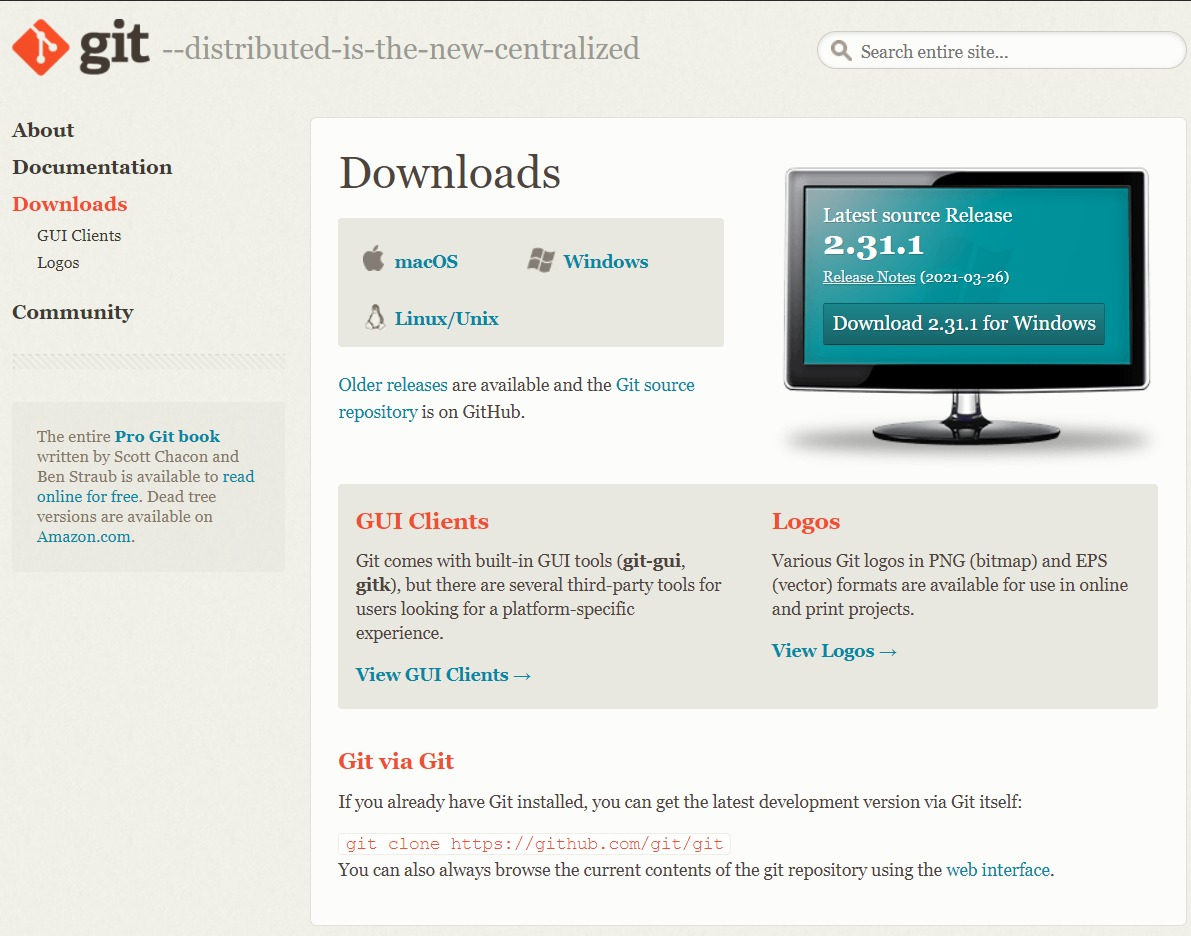
\includegraphics[width=0.70\textwidth]{./img/ind-from-web.jpeg}
  \label{fig:git-web}
\end{figure}

\subsection{Windows}
Una vez descargado el git hay que ejecutar el programa. Aparecera la siguiente ventana y hay que darle click en el botón Ejecutar:
\begin{figure}[H]
  \centering
  \caption{ejecutar programa git}
  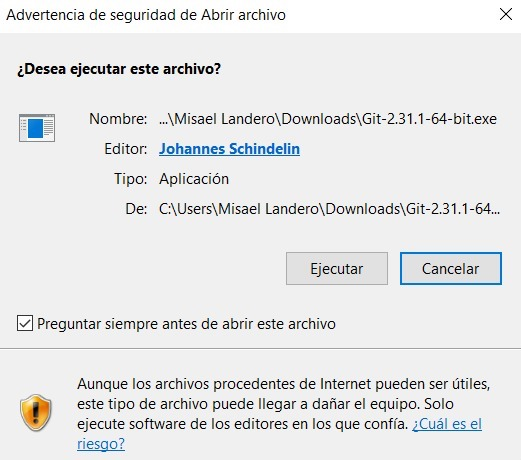
\includegraphics[width=0.50\textwidth]{./img/win/ins-win-1.jpeg}
  \label{fig:git-ins-1}
\end{figure}

Luego se arbrira la ventana de instalación, en la cual le daremos siguiente a la mayoría de las opciones.

\begin{figure}[H]
  \centering
  \caption{ejecutar programa git}
  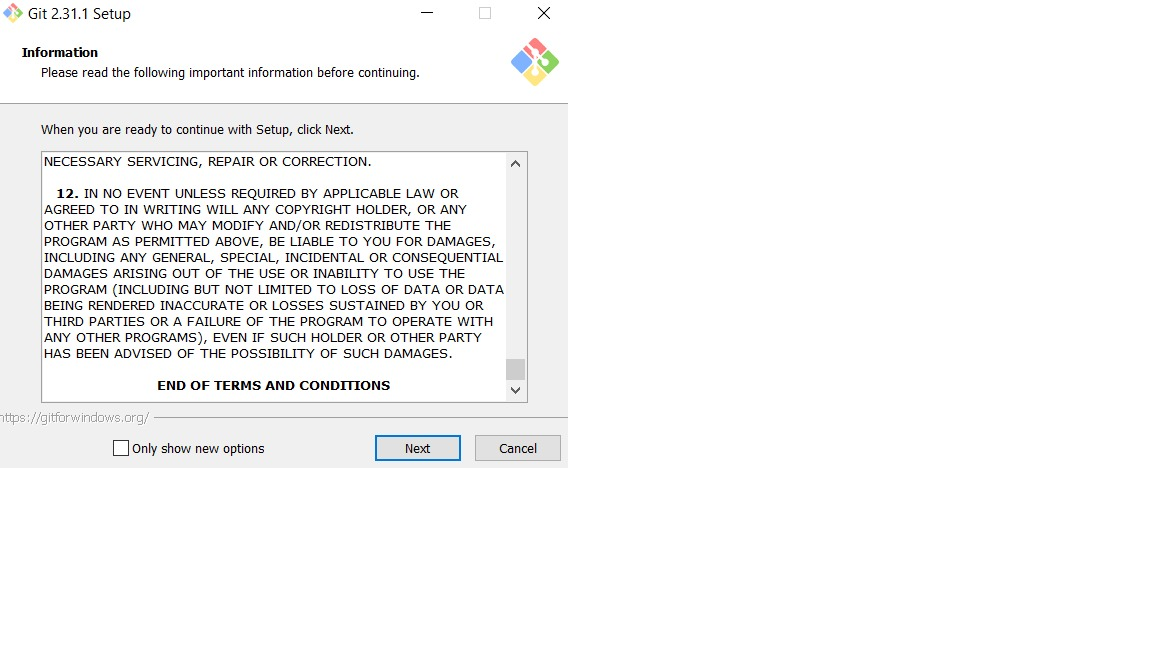
\includegraphics[width=0.50\textwidth]{./img/win/ins-win-2.jpeg}
  \label{fig:git-ins-2}
\end{figure}

Luego de darle click a siguiente una cuantas veces llegaremos a una opción par definir el nombre por defecto de la rama principal, este lo cambiaremos a main en lugar de master ya que GitHub cambió su configuración para que la rama principal se llame main. De esta forma nos ahorraremos cambiarle el nombre a la rama maualmente.

\begin{figure}[H]
  \centering
  \caption{ejecutar programa git}
  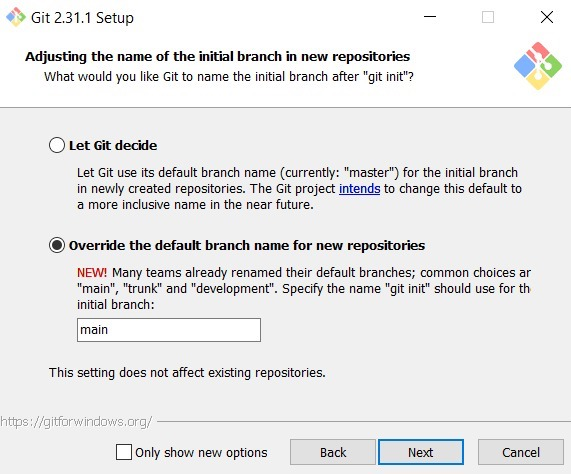
\includegraphics[width=0.50\textwidth]{./img/win/ins-win-3.jpeg}
  \label{fig:git-ins-3}
\end{figure}

La siguiente opción que tendremos que modificar es desde donde podemos ejecutar git, eligiremos la opción de ejecutarlo desde la linea de comando y desde software de terceros (esto nos facilitará usarlo).

\begin{figure}[H]
  \centering
  \caption{ejecutar programa git}
  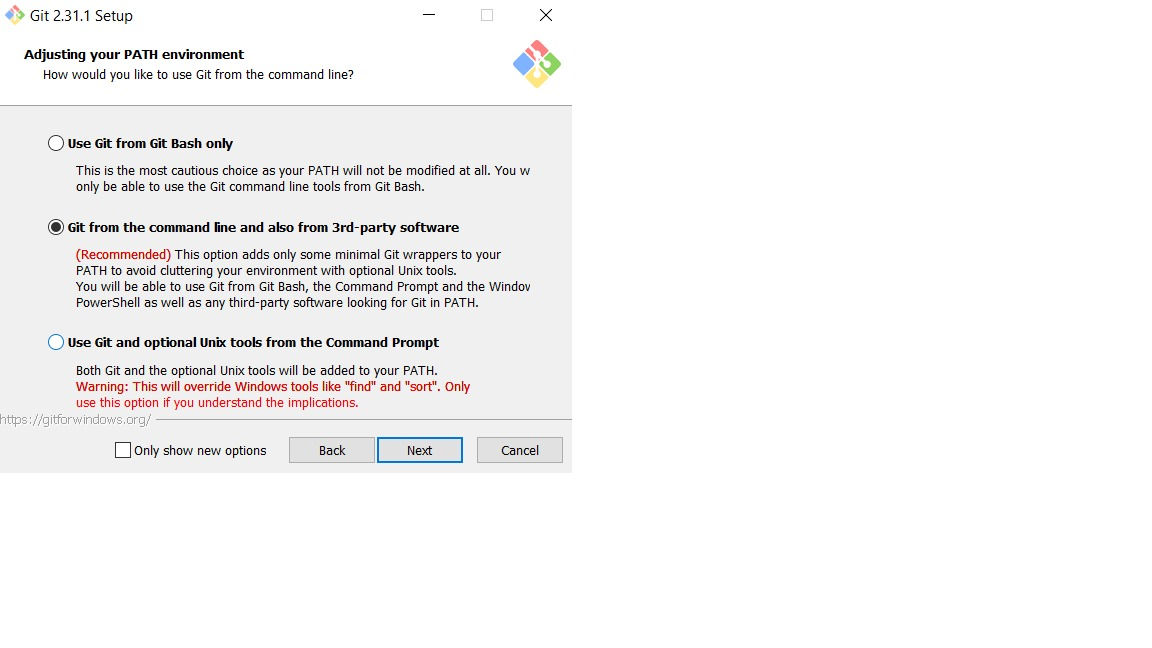
\includegraphics[width=0.50\textwidth]{./img/win/ins-win-4.jpeg}
  \label{fig:git-ins-4}
\end{figure}

La última opción que tenemos que agregar es el de usar pseudo consolas, esto ayuda a poder ejecutar comandos de python o node desde la consoloa de git.

\begin{figure}[H]
  \centering
  \caption{ejecutar programa git}
  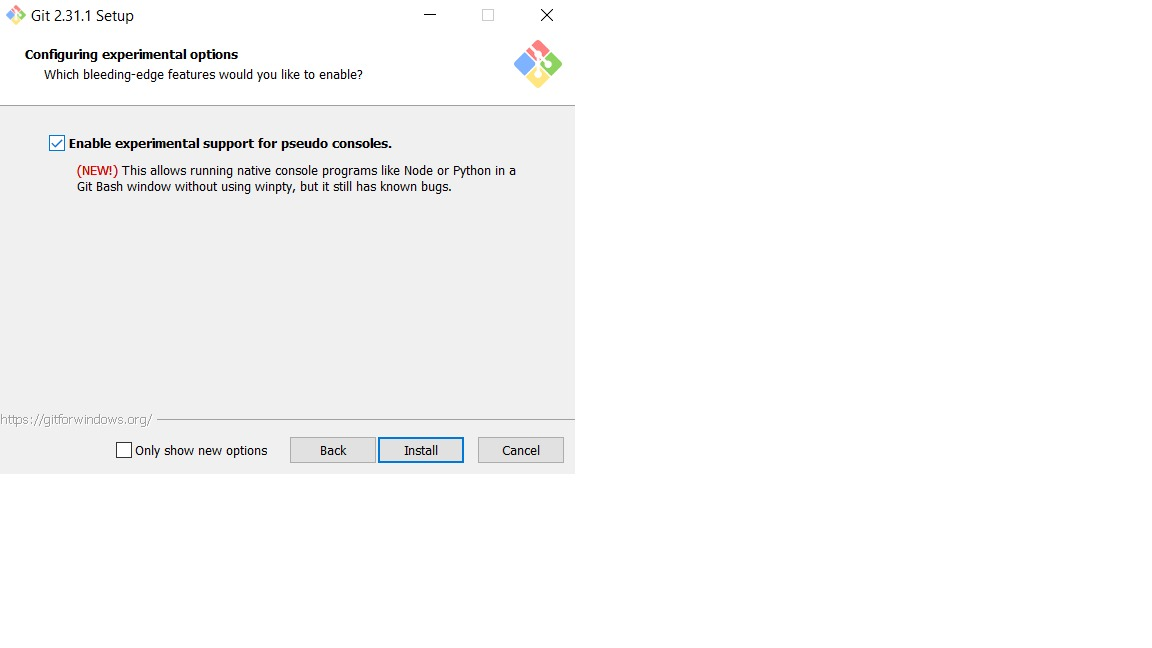
\includegraphics[width=0.50\textwidth]{./img/win/ins-win-5.jpeg}
  \label{fig:git-ins-5}
\end{figure}

Despues de seleccionar la opción anterior le damos click en el botón Instalar y con esto ya tendremos git instalado.

\subsection{Mac}
La instalación de git en mac es mucho mas sencilla, pero antes de poder instalarlo tendremos que instalar un manejador de paquetes. El manejador que paquetes que instalaremos se llama HomeBrew, esta dispobible en el siguiente enlace: \url{https://brew.sh/}.

Para instalar HomeBrew tendremos que abrir el terminal de Mac y escribir el siguiente comando:

\begin{lstlisting}[language=bash,caption={Comando para instalar HomeBrew}]
/bin/bash -c "$(curl -fsSL https://raw.githubusercontent.com/Homebrew/install/HEAD/install.sh)"
\end{lstlisting}

Una vez instalado HomeBrew, instalar git es sencillo. Siempre en el terminal escribiremos el siguiente comando:

\begin{lstlisting}[language=bash,caption={Comando para instalar git en Mac}]
brew install git
\end{lstlisting}

\subsection{Linux}
Por último, instalar git en Linux es mas facil que en los sistemas operativos anteriores. Primero abriremos el termial y luego dependiendo de la distribución de Linux que usemos escribiremos el siguiente comando:

\subsubsection{Ubuntu/Debian}
\begin{lstlisting}[language=bash,caption={Comando para instalar git en Ubuntu}]
apt-get install git
\end{lstlisting}

\subsubsection{Fedora}
\begin{lstlisting}[language=bash,caption={Comando para instalar git hasta Fedora21}]
yum install git
\end{lstlisting}

\begin{lstlisting}[language=bash,caption={Comando para instalar git en Fedora22 y superiores}]
dnf install git
\end{lstlisting}

Para otras distribuciones de linux revisar el siguiente enlace: \url{https://git-scm.com/download/linux}

\section{GitHub}
Github es una plataforma que implemeta Git y hace mas facil poder colaborar con varias personas en proyectos de codigo a traves de la web. GitHub es relativamente sencillo de usar, pero tiene funcionalidades bien robustas para programadores experimentados. 

\subsection{Registrarse en GitHub}
Para empezar a usar GitHub primero hay que crear un perfil en, para esto hay que ir a la dirección web \url{https://github.com/} y hacer click en el botón de la esquina superios izquierda "Sign Up".

\begin{figure}[H]
  \centering
  \caption{Página web de GitHub}
  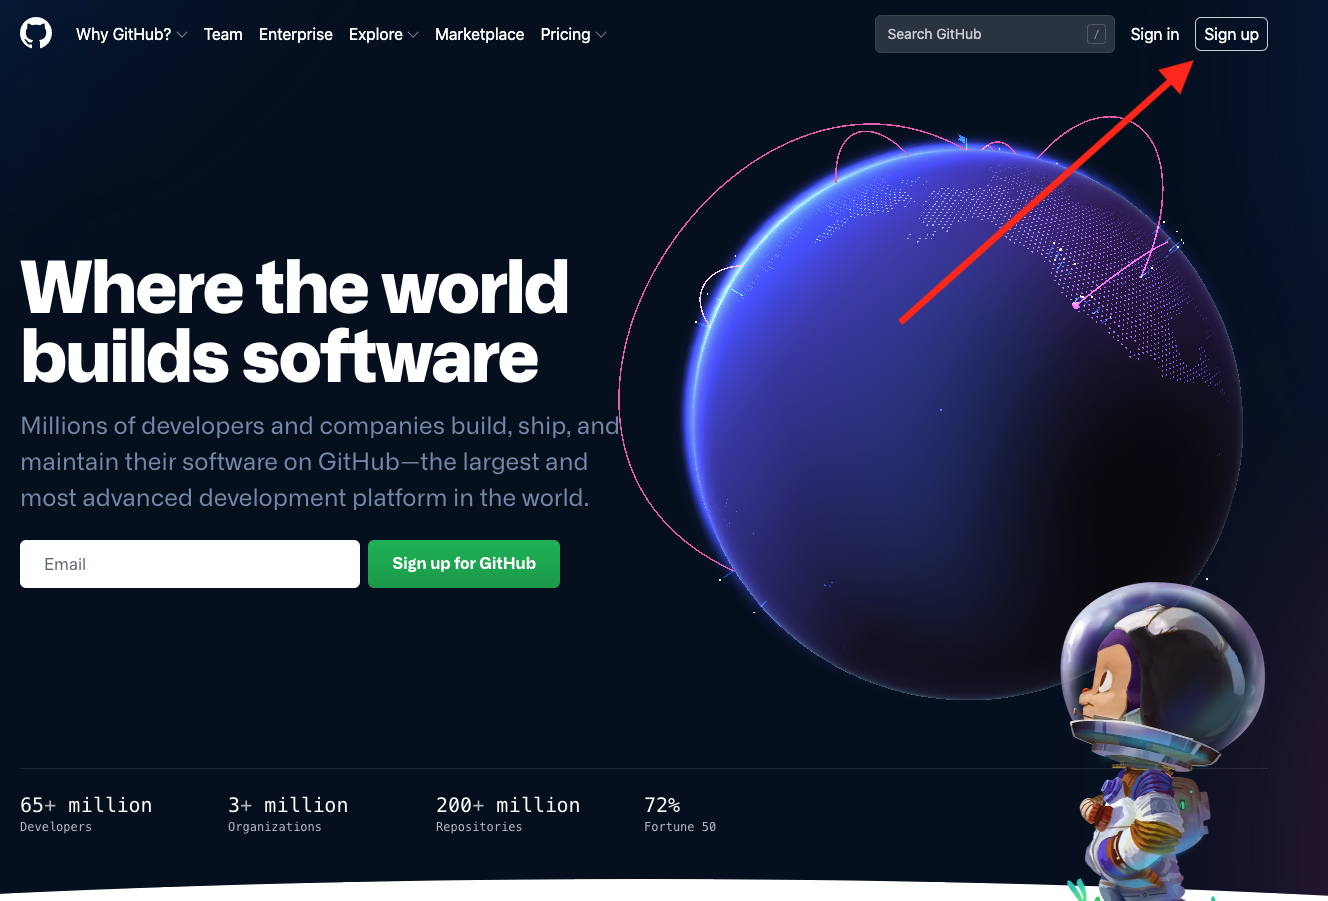
\includegraphics[width=0.90\textwidth]{./img/github-signup-1.png}
  \label{fig:github-signup-1}
\end{figure}

Una vez hayamos dado click en el botón SignUp entratemos a una página donde tendremos que poner nuestros datos para crear la cuenta.

\begin{figure}[H]
  \centering
  \caption{Registrarse en GitHub}
  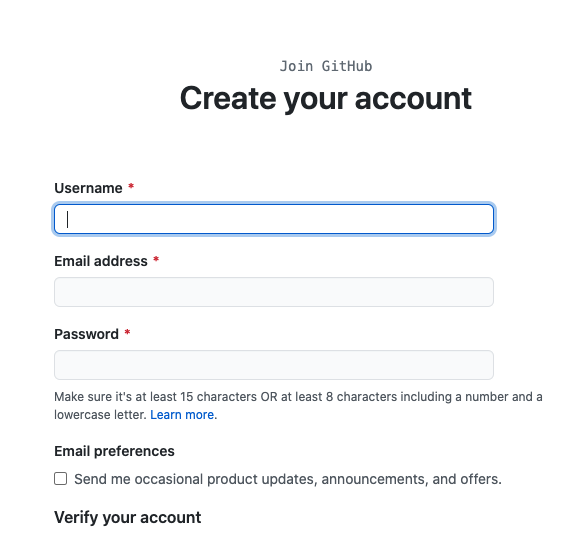
\includegraphics[width=0.50\textwidth]{./img/github-signup-2.png}
  \label{fig:github-signup-2}
\end{figure}

\subsection{Datos de perfil}

Cuando ya tengamos la cuenta deberiamos modificar nuestros datos de perfil ya que GitHun no añade datos como nombre o foto de perfil, si no que hay que ponerlos manualmente. Para agregar estos debemos buscar en la esquina superior derecha un circulo donde debería estar la foto por defecto para nuestro perfil y le damos click.

\begin{figure}[H]
  \centering
  \caption{Configurar perfil}
  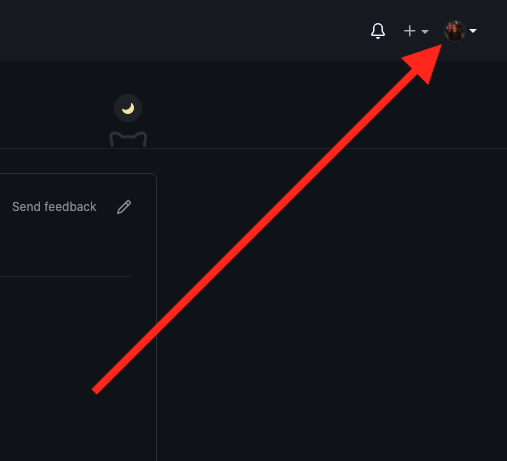
\includegraphics[width=0.50\textwidth]{./img/git-profile-edit.png}
  \label{fig:github-profile-edit}
\end{figure}

Luego de dar click se desplegara un menú y buscamos la opción de configuración ó settings.

\begin{figure}[H]
  \centering
  \caption{Configuración de GitHub}
  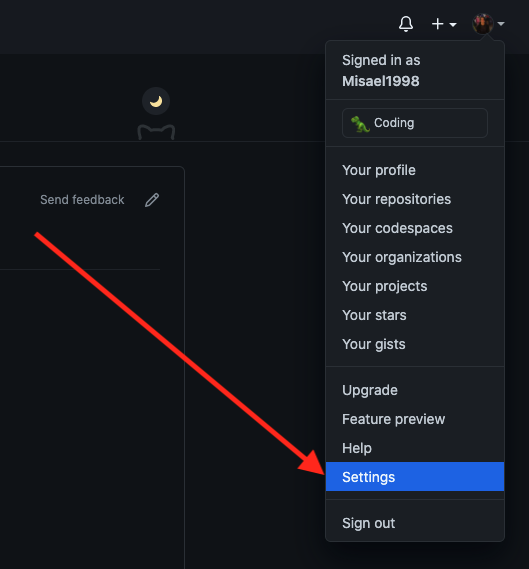
\includegraphics[width=0.50\textwidth]{./img/github-settings-1.png}
  \label{fig:github-settings-1}
\end{figure}

Esto no llevara a la página de configuración de GitHub, en la barra lateral izquierda buscaremos la opción de perfil para poder empezar a agregar nuestros datos.

\begin{figure}[H]
  \centering
  \caption{Configuración de perfil de GitHub}
  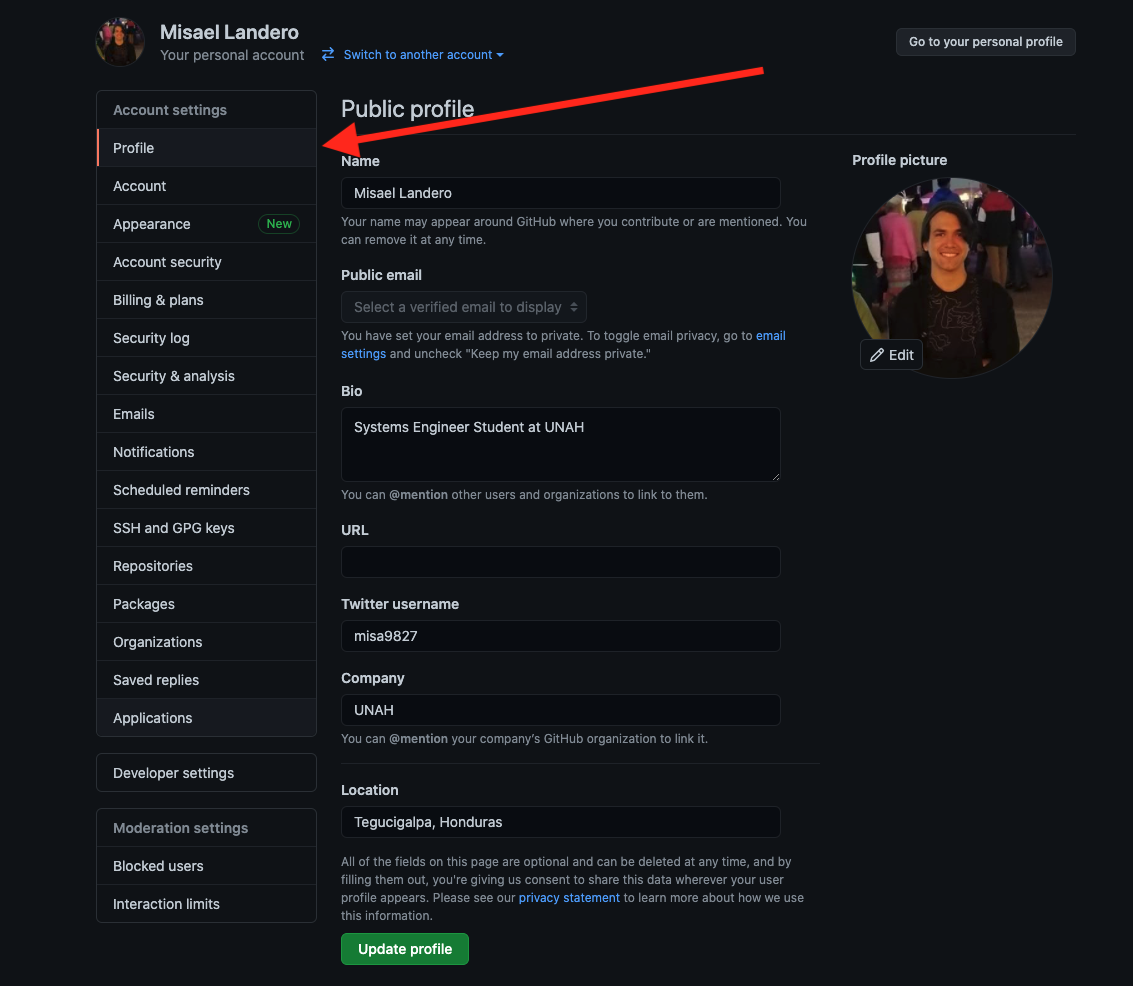
\includegraphics[width=0.50\textwidth]{./img/github-settings-2.png}
  \label{fig:github-settings-2}
\end{figure}

Aquí agregaremos información pública como el nombre, foto de perfil, cuenta de twitter, etc.

Si tenemos un correo de una universidad/institucional lo podemos agregar como correo adicional y esto desbloqueará una plan que normalmente es pagado. Para agregar un correo alternativo buscamos en la barra lateral izquierda la opción de correo ó emails y le damos click. Allí podemos agregar correos adicionales y elegir la visibilidad de estos mismos en nuestro perfil.

\begin{figure}[H]
  \centering
  \caption{Configuración de correo de GitHub}
  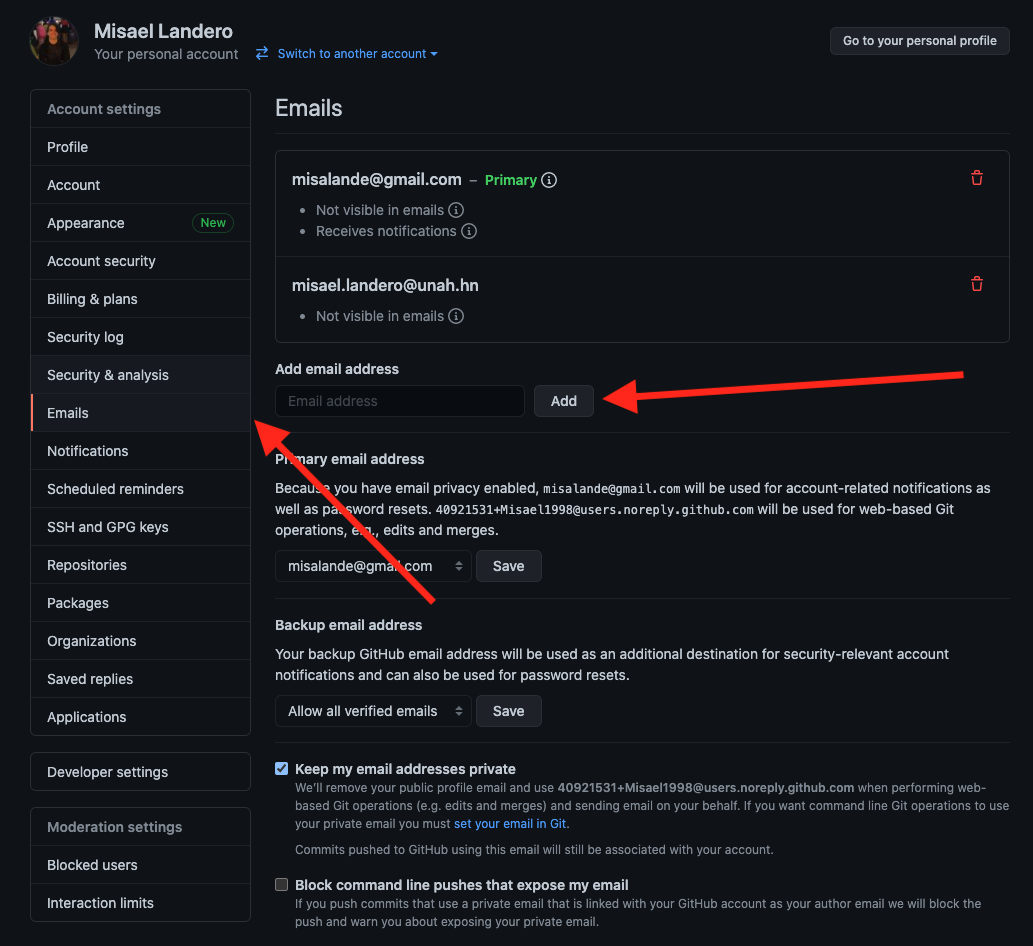
\includegraphics[width=0.50\textwidth]{./img/github-settings-3.png}
  \label{fig:github-settings-3}
\end{figure}

\subsection{Tokens de autenticación}

La última configuración que hay que hacer en GitHub es la de el token de autenticación, esto nos permitira subir nuestros repositorios y cambios hechos en nuestras compuradoreas. Anteriormente GitHub usaba correo y contraseña para autenticación, pero lo están cambiando a tokens con el proposito de hacer más segura la comunicación. Existen otras técnicas como SSH pero los tokens son más faciles de usar. Para empezar a usar los tokens tenemos que entrar en las herramientas de desarrollador que están en la barra lateral izquierda.

\begin{figure}[H]
  \centering
  \caption{Configuración de desarrollador}
  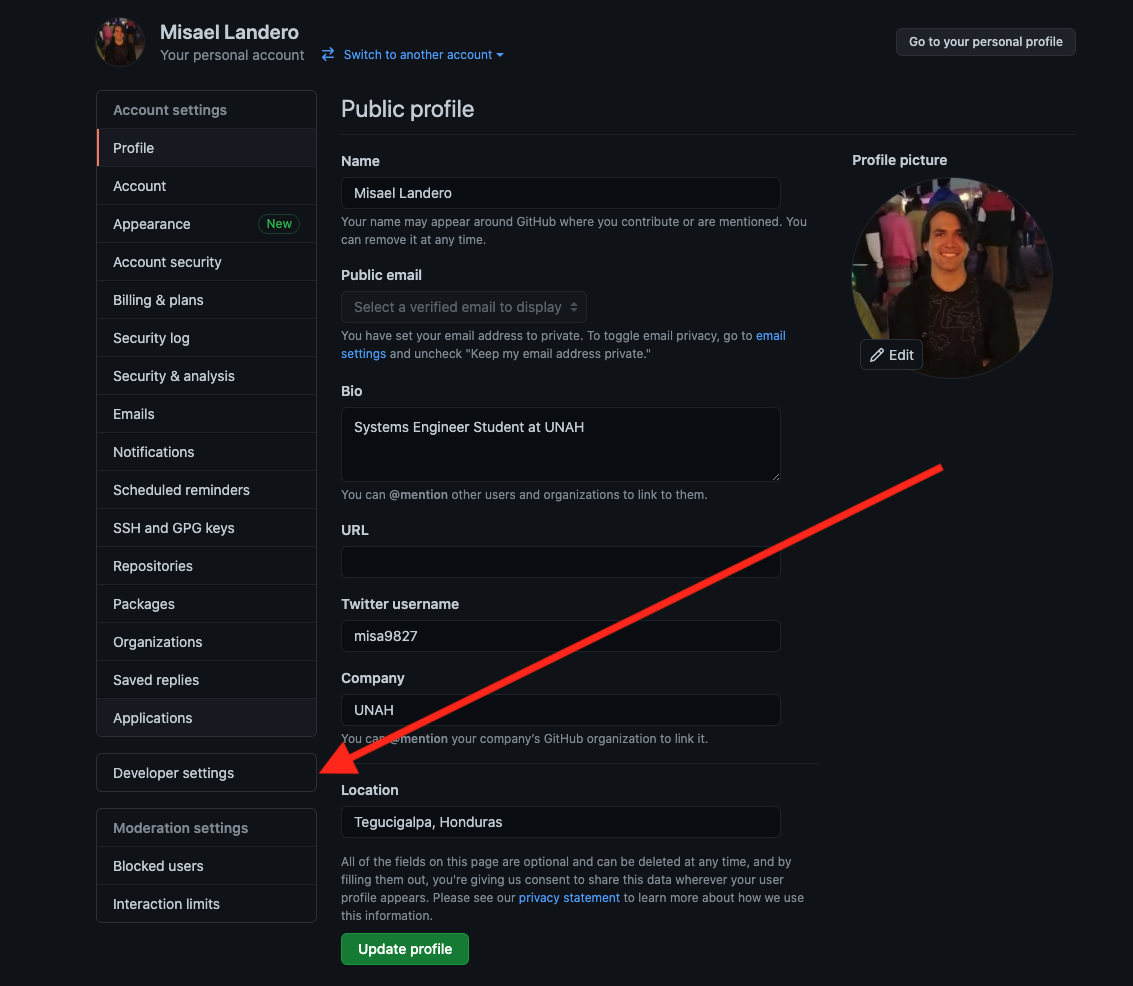
\includegraphics[width=0.50\textwidth]{./img/github-tokens-1.png}
  \label{fig:github-tokens-1}
\end{figure}

Luego buscamos la opción de tokens personales en la barra lateral izquierda y le damos click. Luego le damos click al botón de generar token para crear nuestro primer token.

\begin{figure}[H]
  \centering
  \caption{Tokens}
  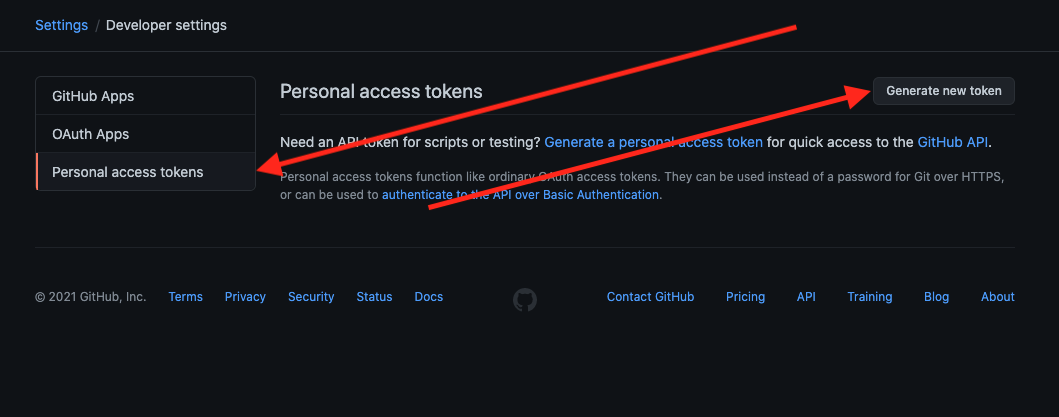
\includegraphics[width=0.70\textwidth]{./img/github-tokens-2.png}
  \label{fig:github-tokens-2}
\end{figure}

Luego hay que seleccionar lor permisos que tendrá el token, para efectos de simplicidad solo seleccionaremos repo. Junto con esto podemos escribir una breve descripción del proposito del token.

\begin{figure}[H]
  \centering
  \caption{Permisos de token}
  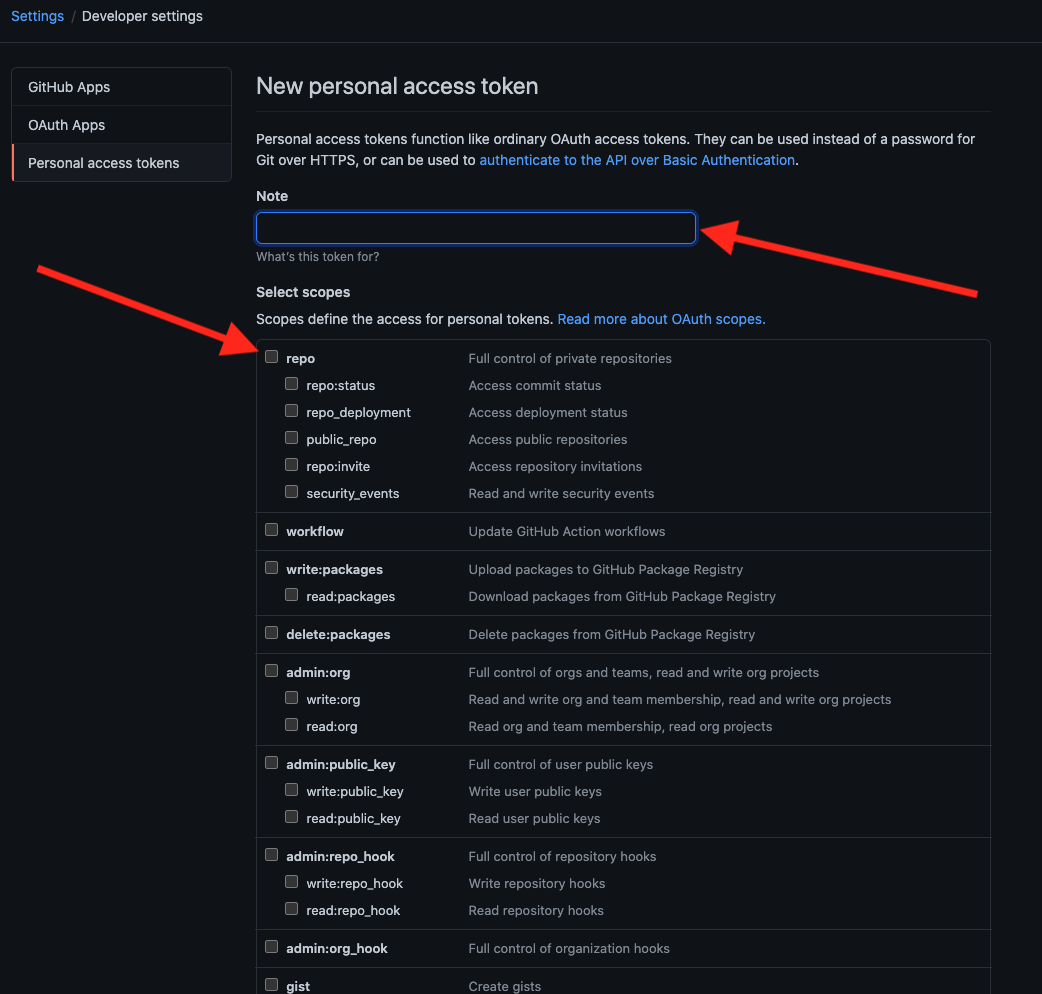
\includegraphics[width=0.50\textwidth]{./img/github-tokens-3.png}
  \label{fig:github-tokens-3}
\end{figure}

Una vez creado el token tenemos que asegurarnos de copiarlo y guardarlo en un lugar seguro, ya que este token es el acceso a los repositorios en los que estamos trabajando. En caso de perder el token se puede simplemente borrar y crear uno nuevo, esta es la ventaja de usar tokens ya que no perdemos acceso a nuestra cuenta en GitHub y no configuramos llaves SSH desde cero.

\begin{figure}[H]
  \centering
  \caption{Token generado}
  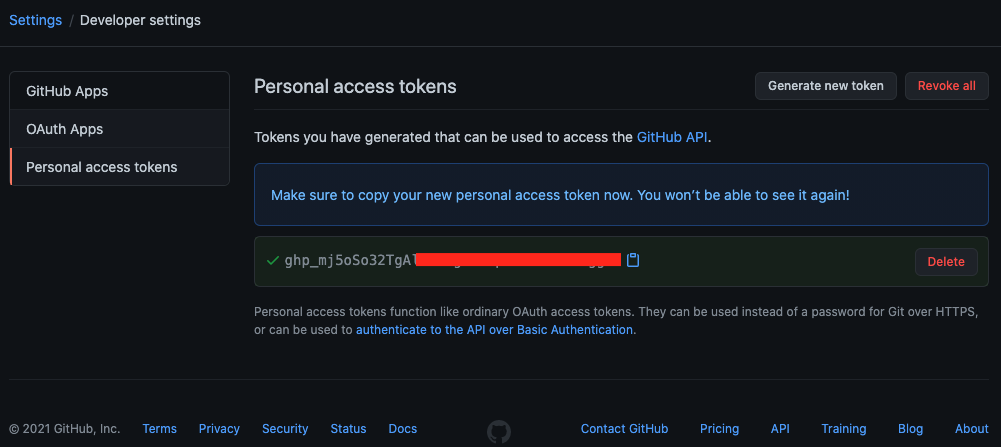
\includegraphics[width=0.70\textwidth]{./img/github-tokens-4.png}
  \label{fig:github-tokens-4}
\end{figure}

\section{Repositorios}
Un repositorio es donde guardamos el proyecto, se podría decir que es una convención que se usa para indicar que una carpeta o directorio contiene cierto tipo de archivos o proyectos. Para que Git empiece a llevar un registro de los cambios en el proyecto lo primero que tenemos que hacer es inicializar un repositorio, hay muchas formas para inicializar un repositorio y cada una puede ser util en diferentes ocaciones pero al final todas hacen lo mismo. Una de las formas mas convenientes es crearlo en GitHub y despues descargarlo, de esta forma podemos definir varias configuraciones del repositorio sin tener que usar el terminal o crear ciertos archivos directamente. 

\subsection{Crear repositorio en GitHub}

Para crear el repositorio en GitHub tenemos que buscar el botón [ + ] en la esquina superior derecha, luego le damos click y seleccionamos nuevo repositorio.

\begin{figure}[H]
  \centering
  \caption{Crear nuevo repositorio}
  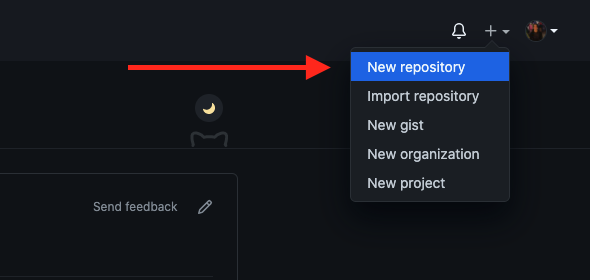
\includegraphics[width=0.70\textwidth]{./img/github-new-repo-1.png}
  \label{fig:github-new-repo-1}
\end{figure}

Esto nos llevará a un menú de configuración para el repositorio, lo primero que haremos sera nombrarlo. Para nombrar un repositorio tenemos que seguir ciertas restricciones como, solo letras minusculas, no se aceptan espacios, el nombre tiene que ser único dentro de nuestros repositorios, etc.

\begin{figure}[H]
  \centering
  \caption{Nombrar repositorio}
  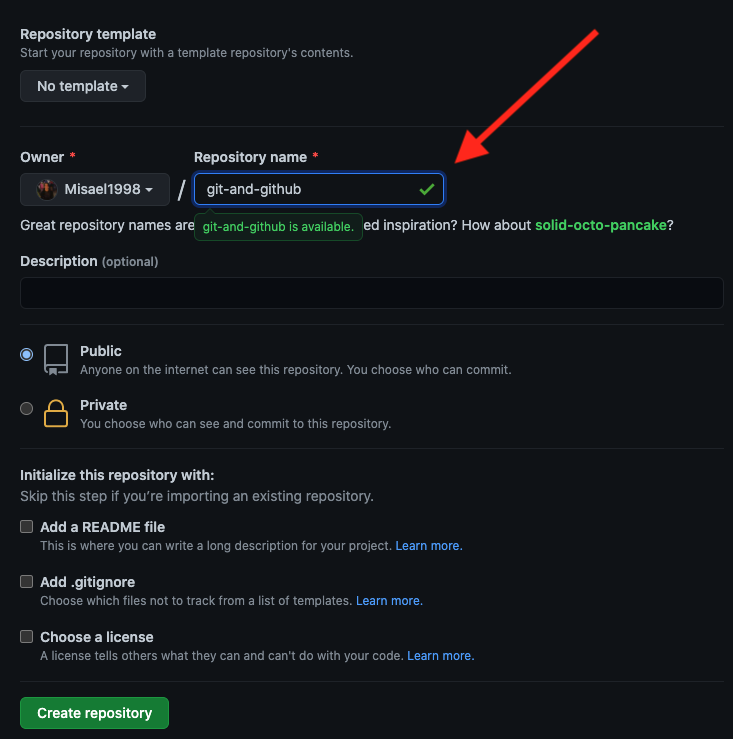
\includegraphics[width=0.70\textwidth]{./img/github-new-repo-2.png}
  \label{fig:github-new-repo-2}
\end{figure}

Si tenemos multiples usuarios ó formamos parte de varias organizzaciones tendremos que especificar quien es el dueño del repositorio (las organizaciones las explicare mas adelante), esta opción la encontramos al lado izquierdo del nombre del repositorio.

\begin{figure}[H]
  \centering
  \caption{Dueño del repositorio}
  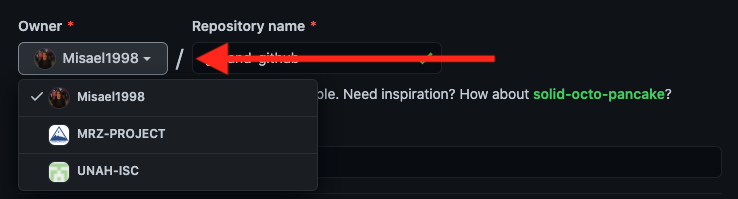
\includegraphics[width=0.70\textwidth]{./img/github-new-repo-3.png}
  \label{fig:github-new-repo-3}
\end{figure}

Luego de esto tenemos la opción de agregar un gitignore, esto sirve para excluir archivos de git i.e. decirle a git cuales archivos no queremos que registre cambios. Para el .gitignore podemos elegir una plantilla para un tipo específico de proyecto, por ejemplo si estamos trabajando en un LaTex podemos buscar la plantilla tex y esto exluira los archivos .log, .dvi, etc. Así git solo se interesa en llevar cambios de los archivos que necesitamos.

\begin{figure}[H]
  \centering
  \caption{.gitignore}
  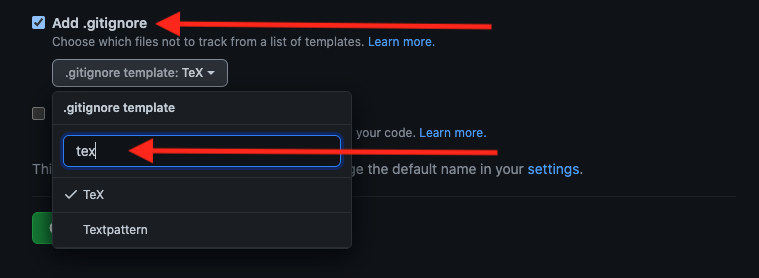
\includegraphics[width=0.70\textwidth]{./img/github-new-repo-4.png}
  \label{fig:github-new-repo-4}
\end{figure}

La siguiente opción que podemos agregar es el uso de una lisencia de software, igual que con la plantilla de .gitignore podemos solo buscar el tipo de lisencia que queremos agregar y marcarla. Aquí podemos agregar de una vez si estamos usando GPL, APACHE, MIT u otras, claro que si cambiamos de lisencia se puede modificar mas adelante.

\begin{figure}[H]
  \centering
  \caption{Lisencias de software}
  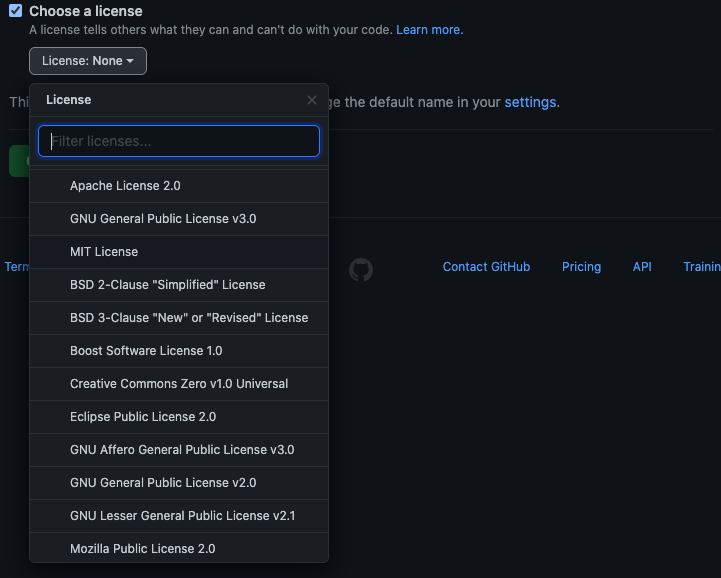
\includegraphics[width=0.70\textwidth]{./img/github-new-repo-5.png}
  \label{fig:github-new-repo-5}
\end{figure}

\subsection{Descargar o clonar un repositorio de GitHub}

Por simplicidad usaremos un entorno gráfico para manejar los repositorios en git, existen varios entornos gráficos para git como GitHub desktop pero usaremos las herramientas de git que tiene integrado VSCode. Primero tenemos que descargar e instalar VSCode, este es un editor de texto asi que la instalación es como la de un programa cualquiera. Descargamos VSCode de la siguiente dirección \url{https://code.visualstudio.com/download} y lo instalamos.

\subsubsection{Clonar repositorios}

Lo primero que tenemos que hacer es buscar el repositorio que queremos clonar en GitHub, si queremos usar un repositorio que creamos en nuestra cuenta lo buscaremos en la sección de repositorios. Esta sección se encuentra en un menú abajo de la barra de navegación.

\begin{figure}[H]
  \centering
  \caption{Repositorios en GitHub}
  
\includegraphics[width=\textwidth]{./img/github-new-repo-6.png}
  \label{fig:github-new-repo-6}
\end{figure}

Esto nos desplegará la lista de los repositorios que tenemos en GitHub, solo buscamos el repositorio que queremos clonar y le damos click para ir a este.

\begin{figure}[H]
  \centering
  \caption{Seleccionar repositorio}
  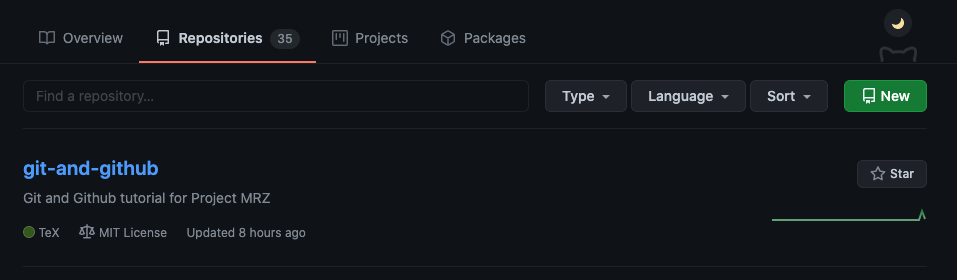
\includegraphics[width=0.70\textwidth]{./img/github-new-repo-7.png}
  \label{fig:github-new-repo-7}
\end{figure}

Una vez que estemos dentro del repositorio en GitHub tenemos que buscar un enlace para clonarlo, para poder encontrar este enlace tenemos que darle click a un botón verde que dice Code ó Codigo. Esto desplegará un pequeño menú y dentro de este aparecera el enlace.

\begin{figure}[H]
  \centering
  \caption{Enlace para clonar repositorio}
  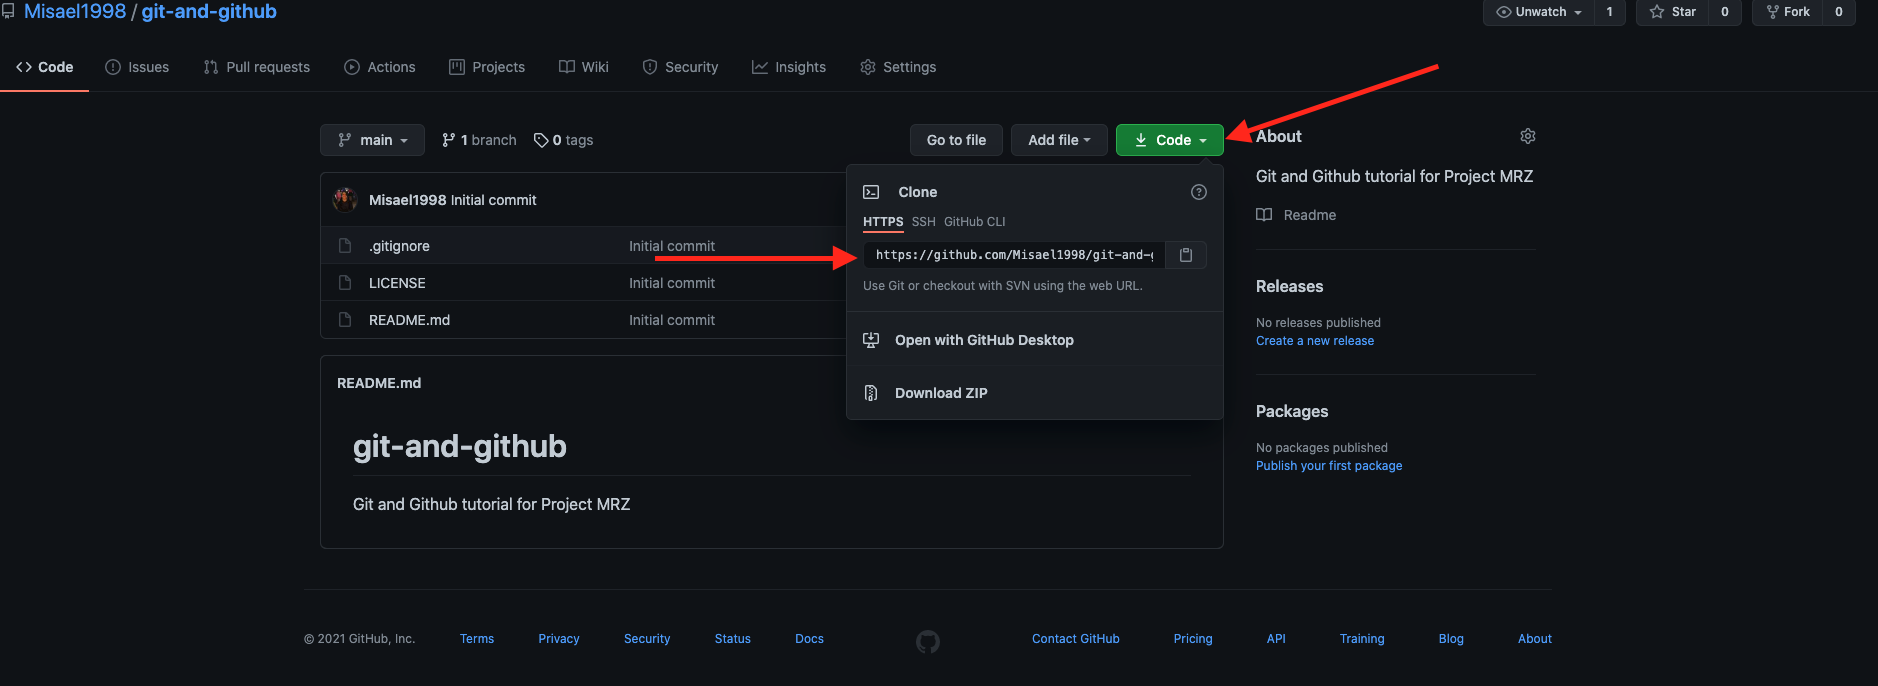
\includegraphics[width=0.95\textwidth]{./img/github-new-repo-8.png}
  \label{fig:github-new-repo-8}
\end{figure}

Ahora nos pasaremos a VSCode, luego de abrirlo haremos click en la primera opción del menú lateral de navevación, en ocaciones ya esta seleccionado por defecto, deberiamos ver una barra lateral con dos botones azules uno para abrir una carpeta y otro para clonar un repositorio. Damos click en el botón de clonar repositorio.

\begin{figure}[H]
  \centering
  \caption{Clonar repositorio desde visual studio code}
  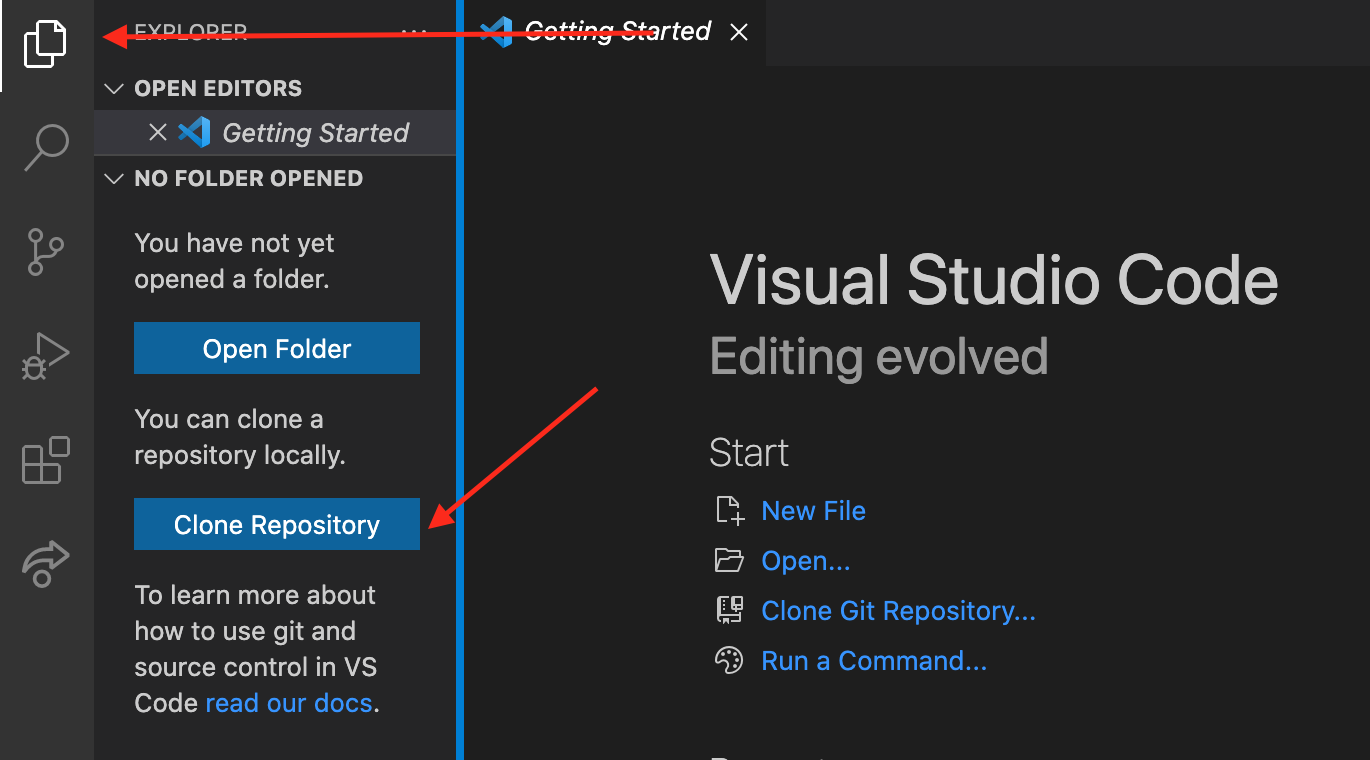
\includegraphics[width=0.70\textwidth]{./img/github-new-repo-9.png}
  \label{fig:github-new-repo-9}
\end{figure}

Luego de apretar el botón nos aparecera una una pequeña barra, en esta pondremos la dirección del repositorio que habiamos copiado en la figura \ref{fig:github-new-repo-8}, luego de pegarlo apretamos la tecla enter.

\begin{figure}[H]
  \centering
  \caption{Colocar url de repositorio}
  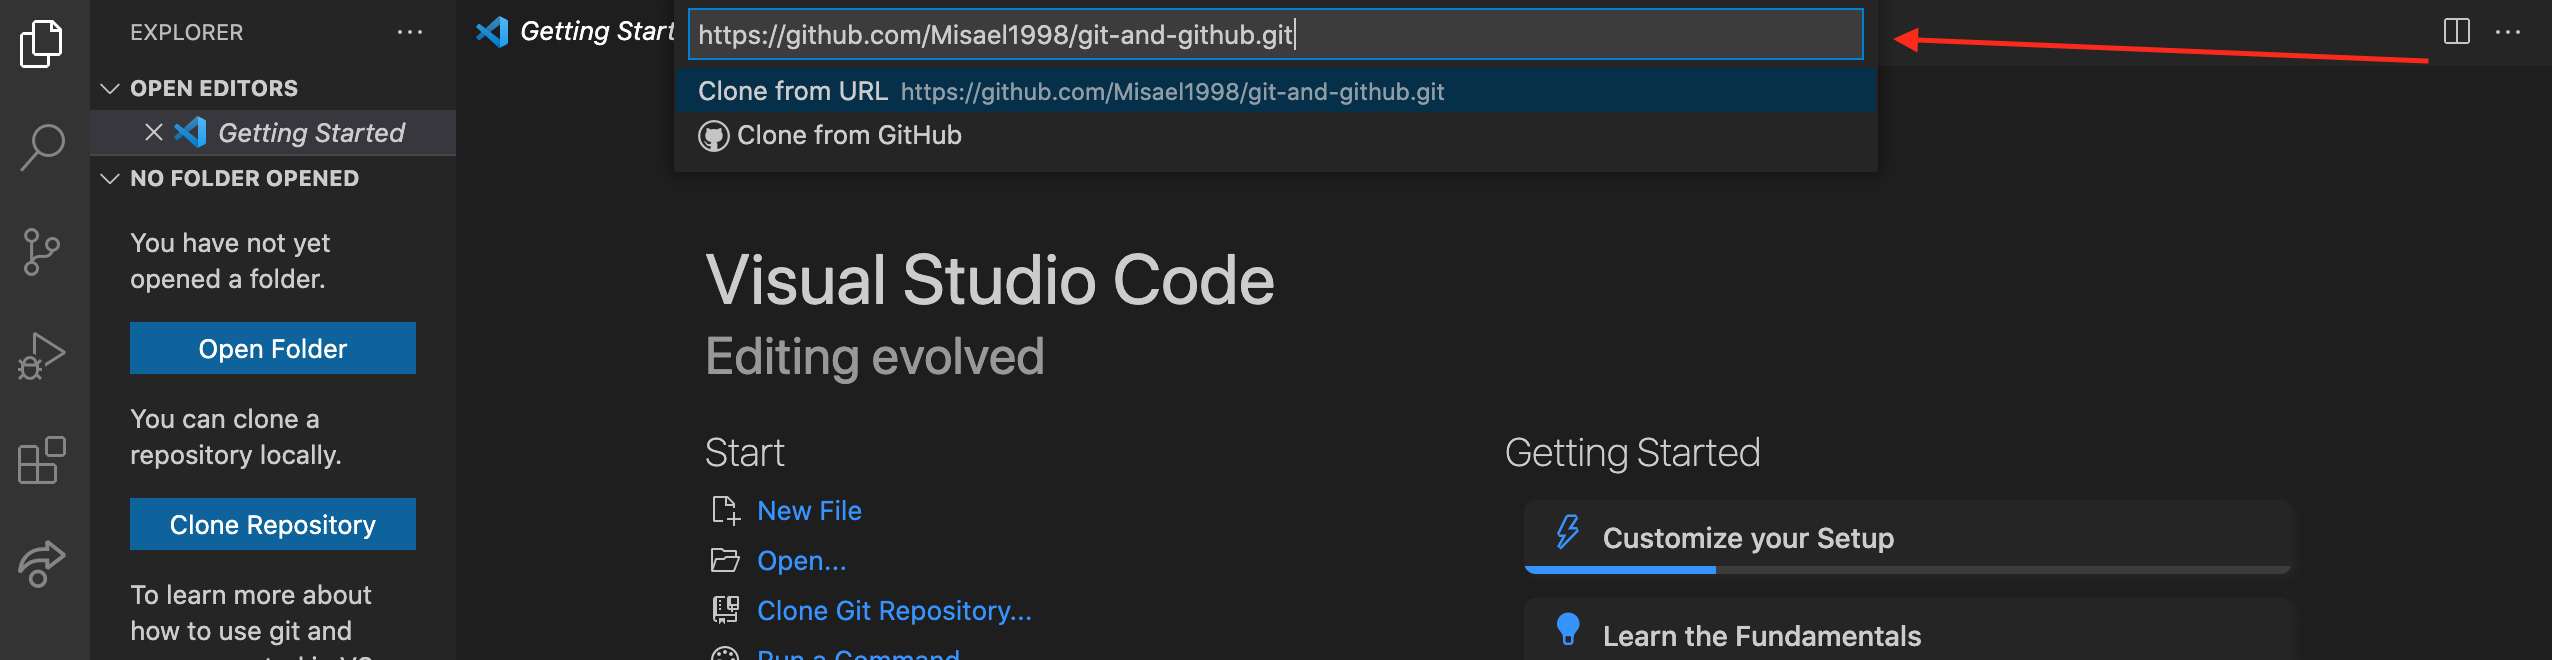
\includegraphics[width=0.70\textwidth]{./img/github-new-repo-10.png}
  \label{fig:github-new-repo-10}
\end{figure}

Despues de hacer esto VSCode nos pedira que seleccionemos una dirección en nuestra computadora para guardar el repositorio. Buscamos el lugar donde queremos guardarlo y le damos click al botón 'Select Repository Location' (este botón podria ser direfente dependiendo del sistema operativo, pero la ubicación no deberia de cambiar significativamente).

\begin{figure}[H]
  \centering
  \caption{Ventana para seleccionar donde guardar el repositorio}
  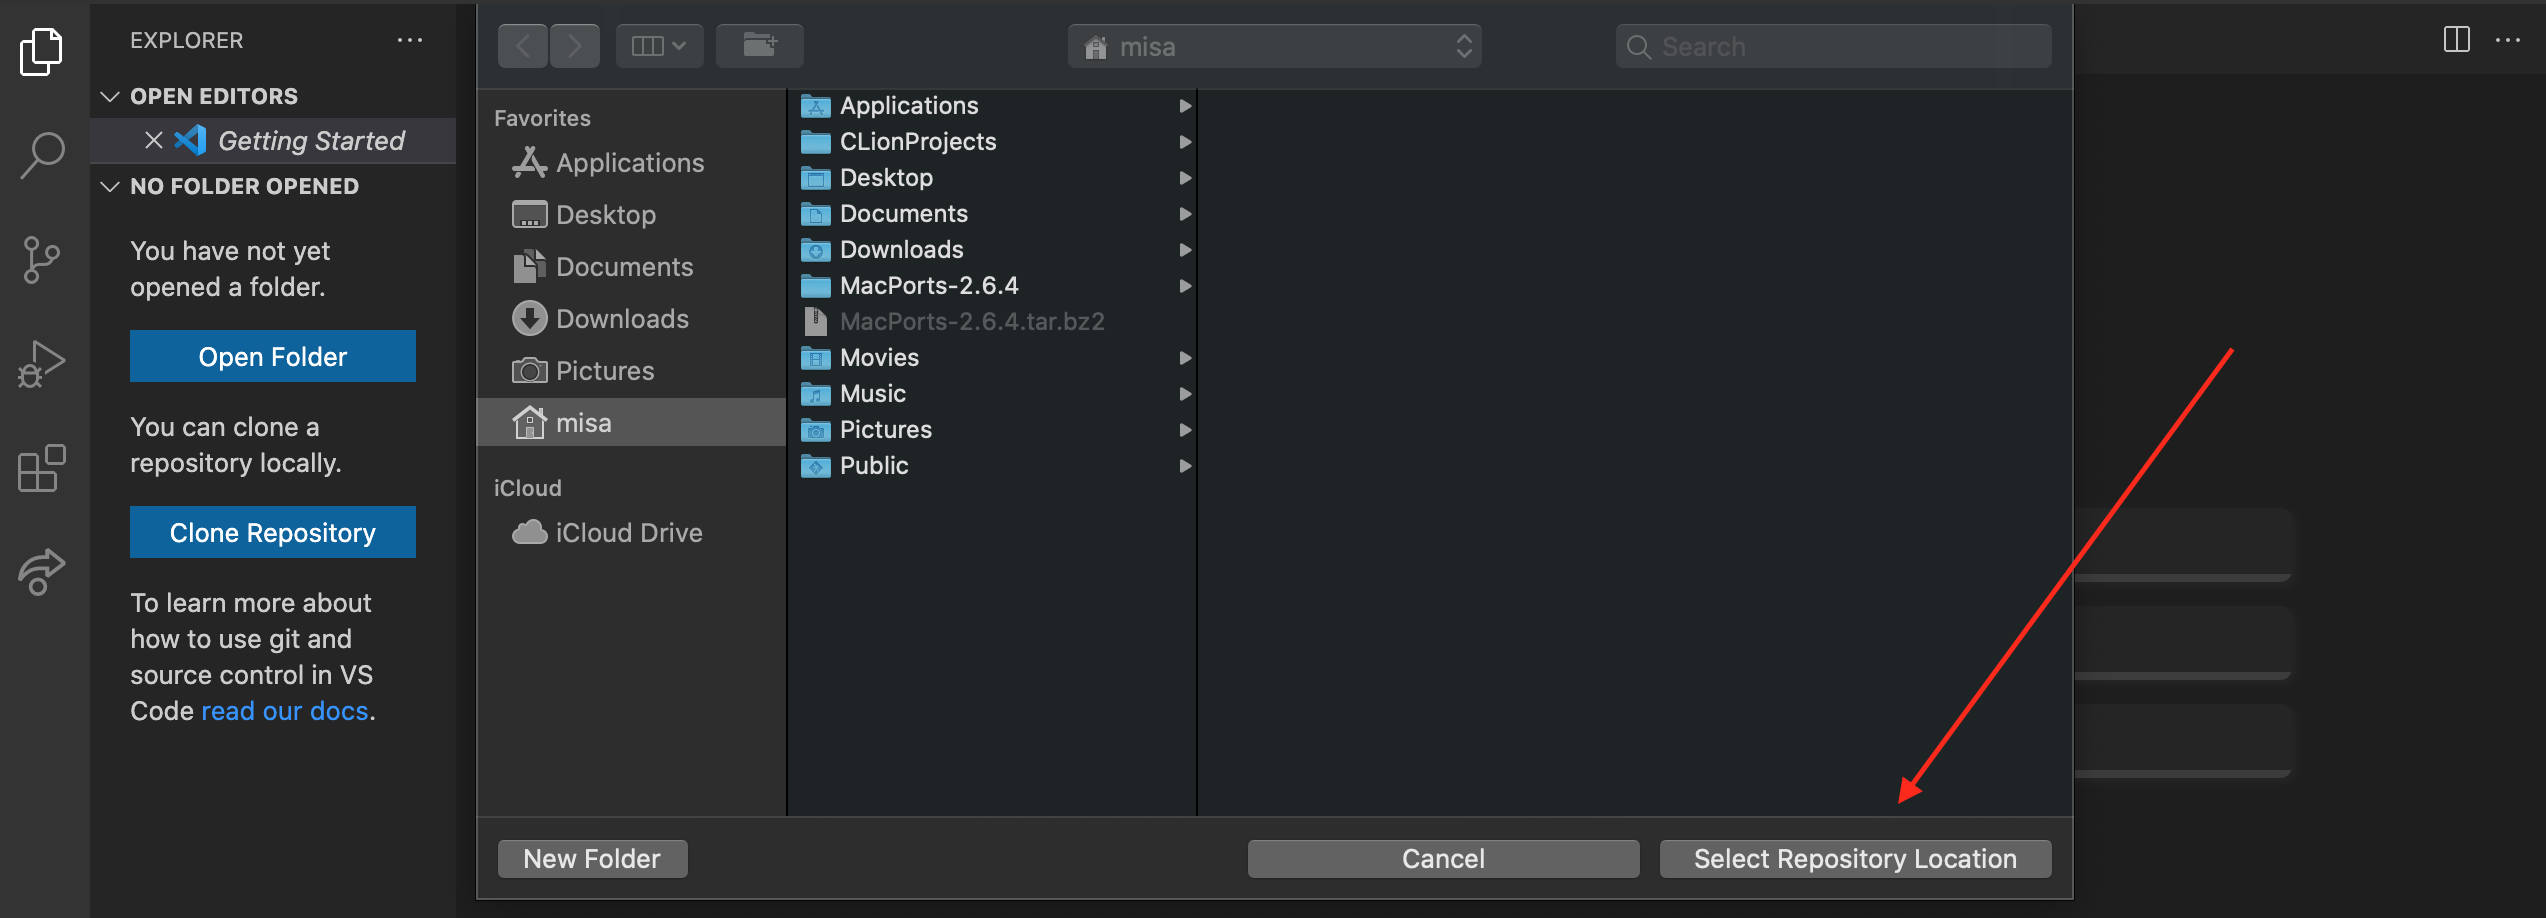
\includegraphics[width=0.70\textwidth]{./img/github-new-repo-11.png}
  \label{fig:github-new-repo-11}
\end{figure}

Una vez descargado el repositorio VSCode nos dara la opción de abrirlos, ahora solo le damos click al botón de abrir y ya podremos ver los contenidos del repositorio dentro de VSCode.

\begin{figure}[H]
  \centering
  \caption{Abrir repositorio una vez descargado}
  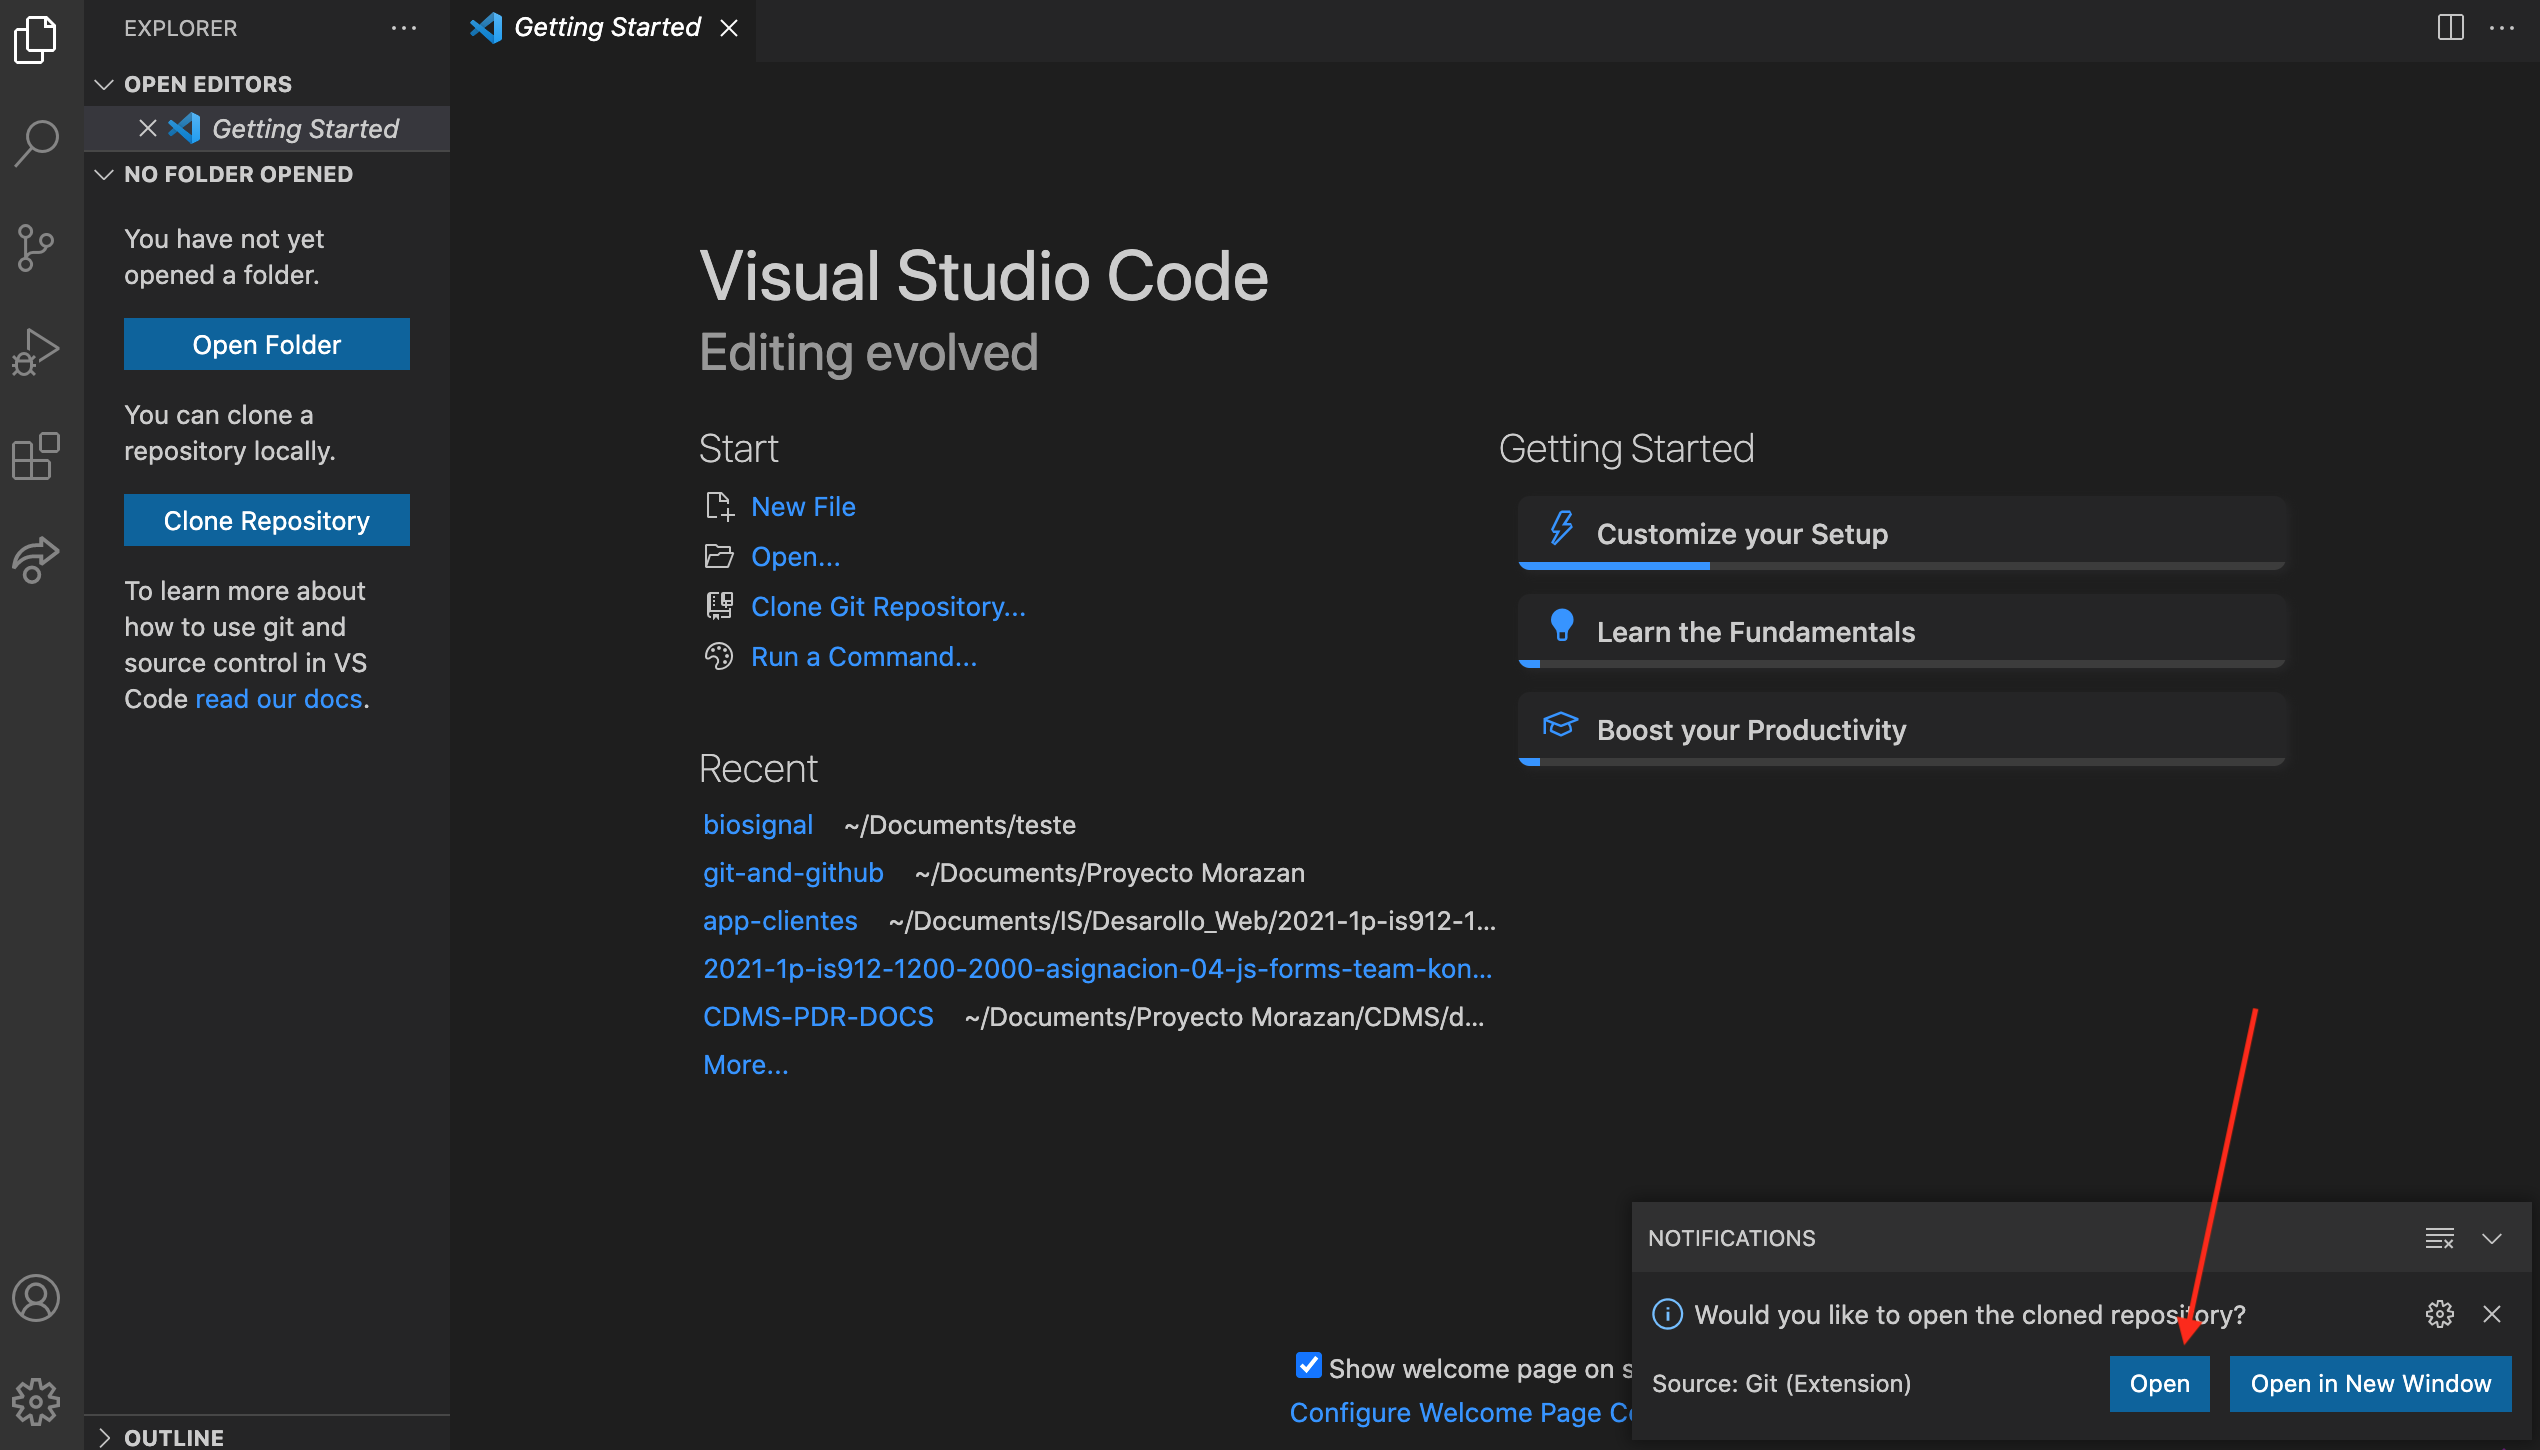
\includegraphics[width=0.70\textwidth]{./img/github-new-repo-12.png}
  \label{fig:github-new-repo-12}
\end{figure}

Con esto todavia no podemos subir nuestro proyecto a GitHub, para eso necesitamos iniciar sesión a traves de VSCode y hacer los primero commits esto lo veremos en la siguiente sección.

\section{Commits}

\section{Branches}

\section{GitHub y Organizaciones}

\end{document}
